\chapter{Программа “Spectral Analyzer PK-4”}
\label{cha:ch_4}
\section{Актуальность программы}
В ходе данной работы был создан веб-сервис “Spectral~Analyzer~PK-4”, название которого состоит из двух частей:
первая часть (“Spectral~Analyzer”) обозначает главную задачу сервиса - спектральный анализ, а вторая часть говорит
о том, что анализ осуществляется на данных, полученных с исследуемой в текущей работе экспериментальной установки
“Плазменный~кристалл-4” (PK-4). Какие задачи решает “Spectral~Analyzer~PK-4”?

Наиболее важная задача - это, собственно, обработка огромного количества спектральной информации, поступающей с борта МКС
Российско-европейской Космической Аппаратуры “Плазменный~кристалл-4”. Поскольку спектральные данные представляют собой
довольно сложную, но упорядоченную структуру данных (см раздел \ref{cha:ch_3_4}), то ручная обработка и
графическое построение даже одного спектра является времязатратной и трудоёмкой задачей: необходимо ориентироваться
в текстовых логах, а также владеть навыками работы, как минимум, с двумя программами одновременно~-~Origin и Exсel.
У умелого пользователя данных программ (при большом желании) получится построить один спектр не быстрее, чем за 5~мин.
Так как в одном эксперименте возможность встретить более 1000~спектров - обычное явление, то даже таких умений становится недостаточно.

Далее, ожидается, что веб-сервис даст инструмент первичной спектральной обработки: полиномиальная калибровка длин волн,
вычитание и усреднение шумового фона, автоопределение пиков спектральных линий, усреднение идентичных спектров при одних
и тех же параметрах и др.

Мотивационный момент, в будущем данный веб-сервис может быть полезен для подготовки датасетов для применения алгоритмов
машинного обучения.

Поскольку в данной работе разработана и применена методика поиска относительного изменения электронной температуры на основе
отношения интенсивностей спектральных линий, то для “Spectral~Analyzer~PK-4” ставится задача рассчета отношений интенсивностей
спектральных линий в зависимости от энергии верхнего уровня.

Еще один мотивационный момент, данный веб-сервис потенциально дает возможность взаимодействовать
с немецкими коллегами по космической аппаратуре ПК-4.

Таким образом, было решено создать автоматизированное компьютеризированное программное обеспечение для решения данных проблем.

\section{Требования к программе}
Чтобы было не только удобно и практично пользоваться и совершенствовать программу, но и для достижения решения
поставленных задач, были выдвинуты определенные требования к программе.

Во первых, программа должна обладать свойством кроссплатформенности, т.е. независимо от типа операционной
системы она должна работать корректно. Конкретнее, должна быть возможность работы под следующими операционными
системами: Windows~XP - Windows~10, MacOs, Linux с графической оболочкой.

Во вторых, программа должна иметь возможность сохранения ключевых состояний процесса обработки данных,
а также максимально безболезненно передавать прогресс между пользователями.

Далее, программа должна уметь в автоматическом режиме загружать и парсить текстовые спектральные данные
(эксперименты), а также отображать список уже загруженных экспериментов.

Следующий важнейший аспект - это умение динамически отображать более 1000~спектральных графиков в одном
рабочем окне, отображать метаинформацию по текущему спектру.

Для обработки спектров необходимо учитывать фоновое излучение, поэтому программа должна иметь возможность по
выбранным пользователем номерам спектров усреднять их интенсивности, а также вычитать из всех спектров текущего эксперимента.

Не менее важный аспект - это возможность настроить калибровку спектра по длине волны на основе вводимой пользователем полиномиальной функции.

Далее, для поиска отношений интенсивностей необходимо на основе откалиброванных незашумленных спектров сохранять
усредненные спектры-заготовки с учётом среднеквадратичных погрешностей, также необходимо отображать
список уже сохранённых усредненных спектров.

В силу того, что используемый спектрометр “OceanOptics~USB2000+” имеет невысокую разрешающую
способность (см раздел \ref{cha:ch_3_4}), то для корректного поиска отношений интенсивностей
необходимо учитывать наложения линий друг на друга с помощью аппаратной функции спектрометра,
т.е. следующее требование к программе: она должна уметь на основе полиномиального приближения аппаратной
функции учитывать перекрытия рядом стоящих линий с учетом погрешностей.

В данной работе особый интерес представляет зависимость отношения интенсивностей определенных линий от энергии
возбужденного состояния, для этого программа должна иметь библиотеку спектральных линий, а также функционал
по выбору набора линий при построении данной зависимости.

Таким образом, мы перечислили основные требования к программе, а сейчас разберем стек технологий,
который был изучен для достижения данных целей (см.~рис.~\ref{fig:it_tech}).
\begin{figure}[t]
  \centering
  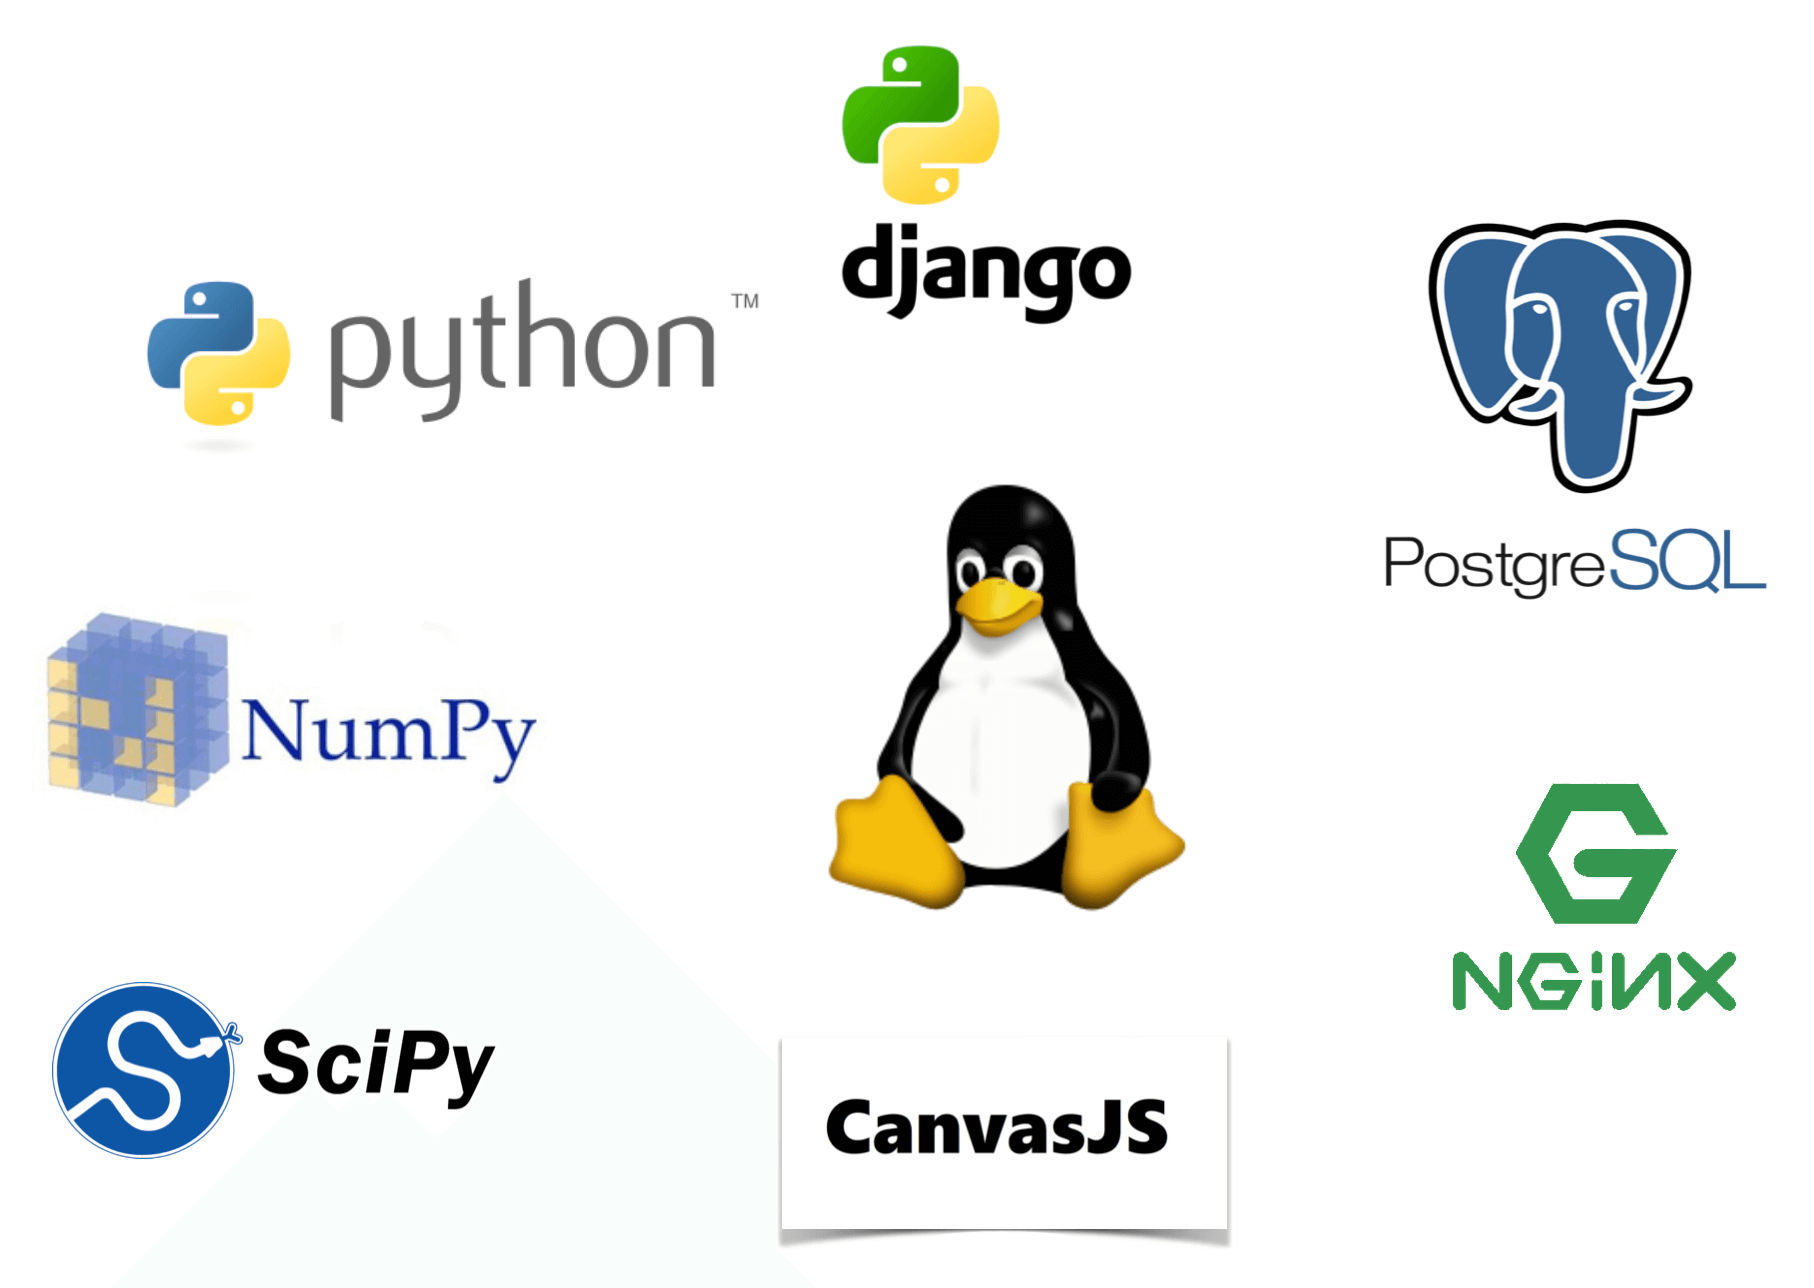
\includegraphics[width=12cm]{figures/it_tech}
  \caption{Изображены логотипы изученных IT-технологий, которые использовались для создания веб-сервиса “Spectral~Analyzer~PK-4”}
  \label{fig:it_tech}
\end{figure}

\section{Стек изученных технологий}
Первый прототип программы был написан традиционным образом на языке C\#, который непременно предполагает
стандартную установку под Windows и работу с программой, как с ПО для данной операционной системы.
В данном варианте было реализовано лишь около 20\% необходимого функционала, но при этом возникли большие трудности
с передачей программы научному руководителю из-за несовместимости версий Windows~7 и XP.

Для решения проблем кроссплатформенности и передачи данных между пользователями было решено создать веб-сервис,
который работает в обычном браузере, поскольку почти каждая операционная система с графической оболочкой
поддерживает большинство современных браузеров.

Django (Джанго)~--~свободный фреймворк для веб-приложений на языке Python, использующий шаблон проектирования MVC.
Проект поддерживается организацией Django Software Foundation \cite{Django}. Джанго имеет удобную гибкую
внутреннюю архитектуру, которая позволяет разработчикам, при достаточных знаниях, выполнять огромный спектр задач
из области веб-программирования. Перечислять все возможности данного фреймворка нет необходимости, подчеркнем лишь те,
что были использованы для решения поставленных задач.

Джанго имеет свою стандартизированную ORM, которая поддерживает транзакции. ORM (англ. Object-Relational Mapping,
рус. объектно-реляционное отображение или преобразование)~--~это некая оболочка над базой данных, которая позволяет
использовать функционал базы данных с помощью объектно-ориентированного языка программирования, в данном случае с помощью Python.

Далее, в Джанго есть система маршрутизации урлов, которая позволяет настраивать POST и GET запросы на основе регулярных выражений,
что очень удобно: в Python есть хорошо известный и понятный встроенный модуль “re”, который почти ничем не отличается по синтаксису.

В Джанго предусмотрена возможность применения криптографически шифрованных Cookie и CSRF-токенов для защиты POST
запросов к серверу: например, для аутентификации пользователя, для любого изменения и некоторых запросов к информации сервера.
Это дает довольно хорошую защиту от мошеннических и хакерских атак.

PostgreSQL~--~свободная объектно-реляционная система управления базами данных, разработанная в Калифорнийском
университете на факультете компьютерных наук в Беркли \cite{PostgreSQL}. PostgreSQL поддерживает большой набор встроенных типов данных:
\begin{itemize}
\item численные типы;
\item двоичные типы;
\item типы «дата/время»;
\item булев тип;
\item перечисление;
\item геометрические примитивы;
\item UUID-идентификатор;
\item XML-данные;
\item массивы;
\item JSON;
\item идентификаторы объектов БД;
\item псевдотипы;
\end{itemize}

NumPy является основным пакетом для научных вычислений в Python, которая поддерживает
многомерные массивы (в~т.ч.~матрицы), а также предоставляет прекрасно оптимизированные высокоуровневые методы для работы с ними,
включая математические, логические, манипуляции с размерностью, сортировку, отбор, ввод-вывод, дискретные преобразования Фурье,
основную линейную алгебру, основные статистические операции, случайное моделирование и многое другое \cite{Numpy}.
Исходный код NumPy находится в открытом доступе.

SciPy — библиотека для языка программирования Python с открытым исходным кодом, предназначенная для выполнения научных и
инженерных расчётов \cite{Scipy}. Возможности:
\begin{itemize}
\item поиск минимумов и максимумов функций;
\item вычисление интегралов функций;
\item поддержка специальных функций;
\item обработка сигналов;
\item обработка изображений;
\item работа с генетическими алгоритмами;
\item решение обыкновенных дифференциальных уравнений;
\end{itemize}

CanvasJS - библиотека для языка программирования JavaScript, которая предоставляет API для работы с диаграммами и графиками
в веб-проектах. Для студентов и некоммерческого использования лицензия предоставляется бесплатно. Основные преимущества:
\begin{itemize}
\item простой API;
\item высокая производительность;
\item 30 типов диаграмм;
\item хорошая документация;
\item поддержка браузеров Chrome, Firefox, Safari, IE8+;
\end{itemize}

При создании веб-сервиса “Spectral~Analyzer~PK-4“ использовались следующие версии библиотек:
\begin{itemize}
\item django==2.0;
\item psycopg2==2.7.1;
\item numpy==1.14.2;
\item django-debug-toolbar==1.8;
\item scipy==1.0.1;
\item python-dateutil==2.6.1;
\item canvas-js==2.1
\end{itemize}

\section{Описание функционала}
Используя описанный стек технологий был создан веб-сервис “Spectral~Analyzer~PK-4” версии 1.0.0.
В данном разделе находится информация о том, как пользователь взаимодействует с сервисом данной версии, описание функционала
и некоторые решения на программном уровне, которые показались автору интересными/полезными для прочтения.

С точки зрения установки данного программного обеспечения все сильно упрощено~--~достаточно лишь открыть URI
сервиса в своем браузере и начать работу. Таким образом пользователь освобождается от трудоемких операций по получению ПО
и может пользоваться сервисом с любой точки мира, почти с любого устройства, имеющего совместимую версию браузера.

Первое взаимодействие с пользователем начинается со страницы аутентификации (см.~рис.~\ref{sub:auth}). На данном
этапе проходит проверка пользователя на наличие доступа к контенту: необходимо ввести почту и пароль, выданные разработчиками
сервиса. На программном уровне пользователь имеет следующую ORM абстракцию:

\begin{figure}[t]
    \begin{center}
         \subfloat[\label{sub:auth}]{
           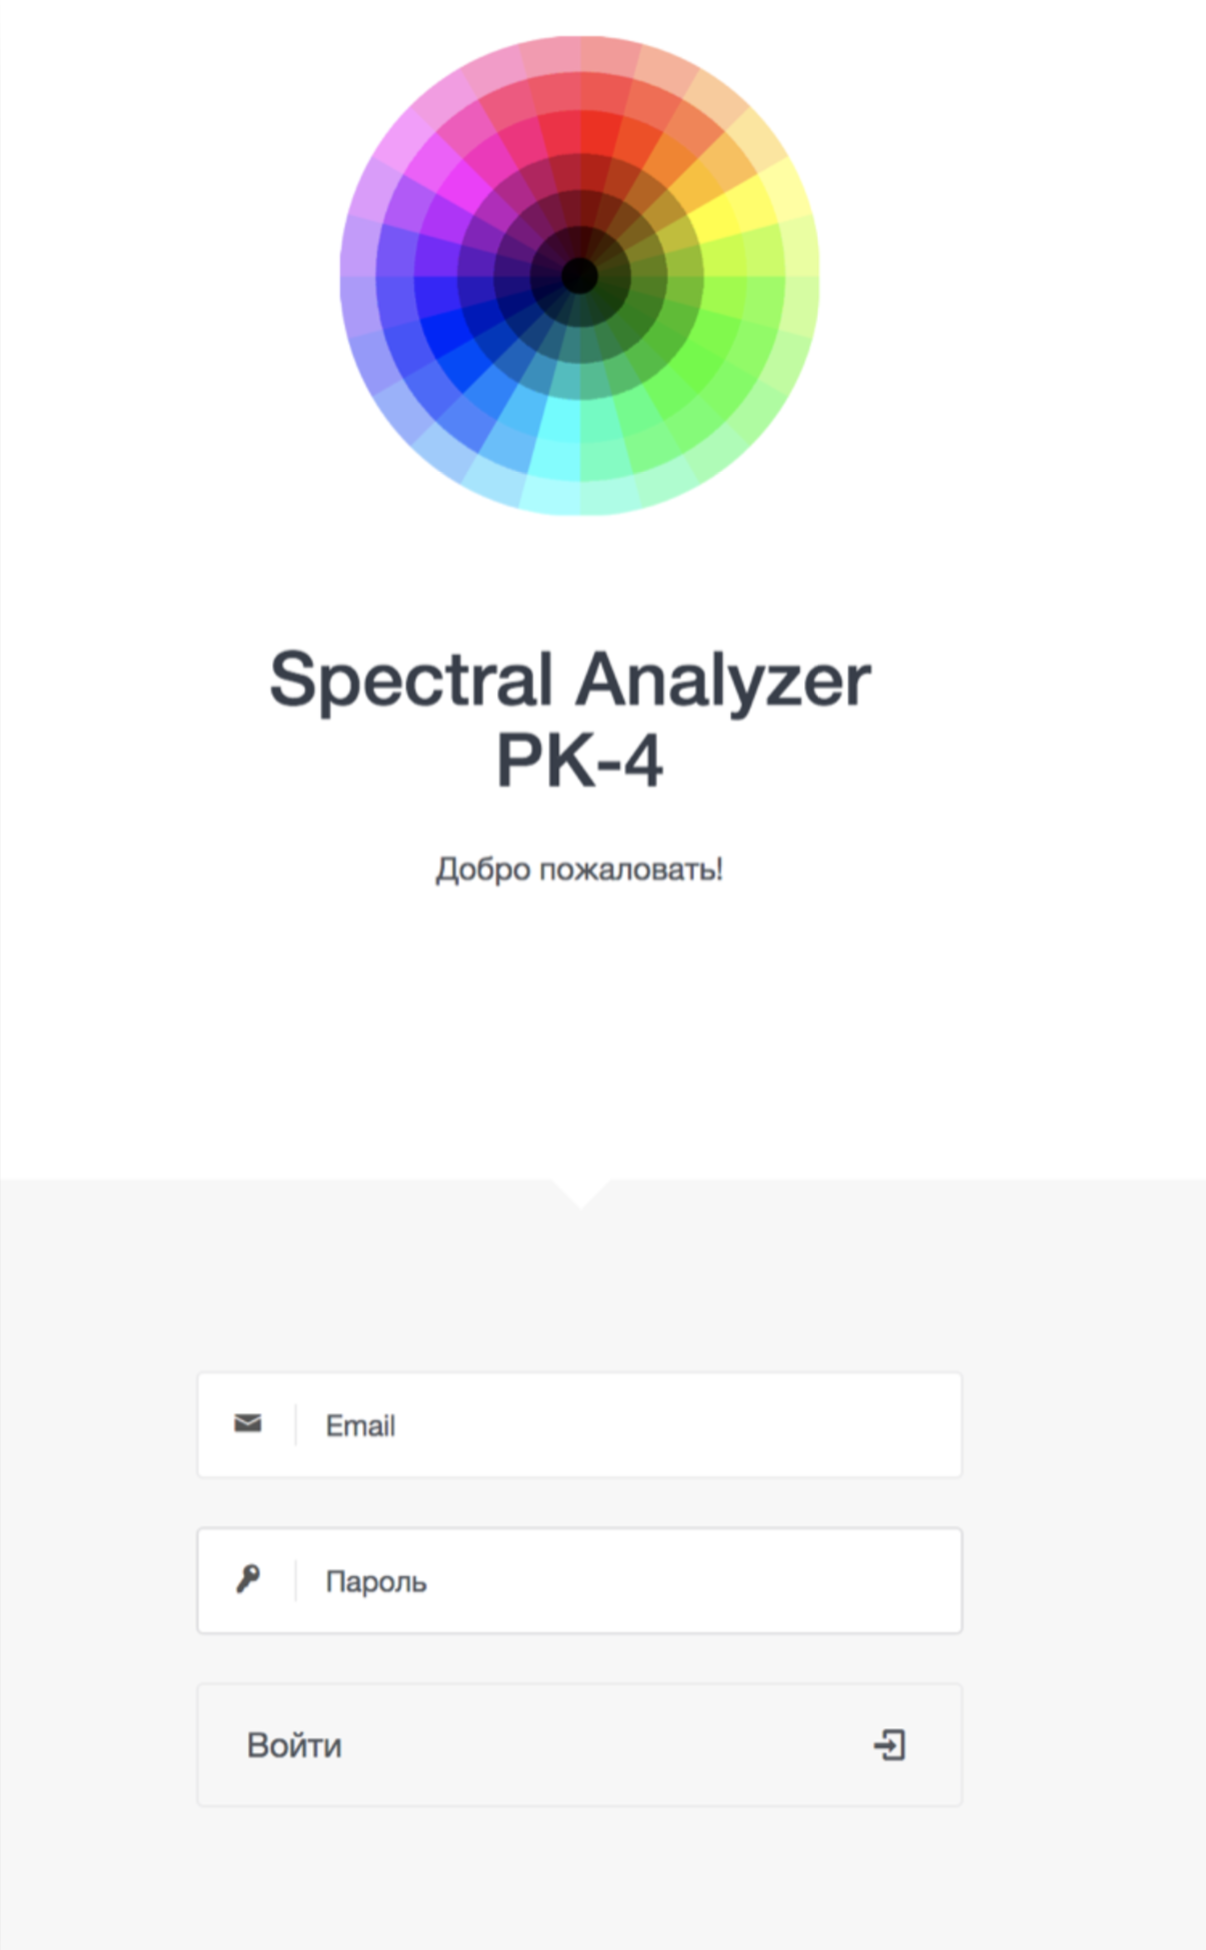
\includegraphics[width=0.35\textwidth]{figures/auth}
         }
         \hspace{0.05\columnwidth}
         \subfloat[\label{sub:page_not_found}]{
           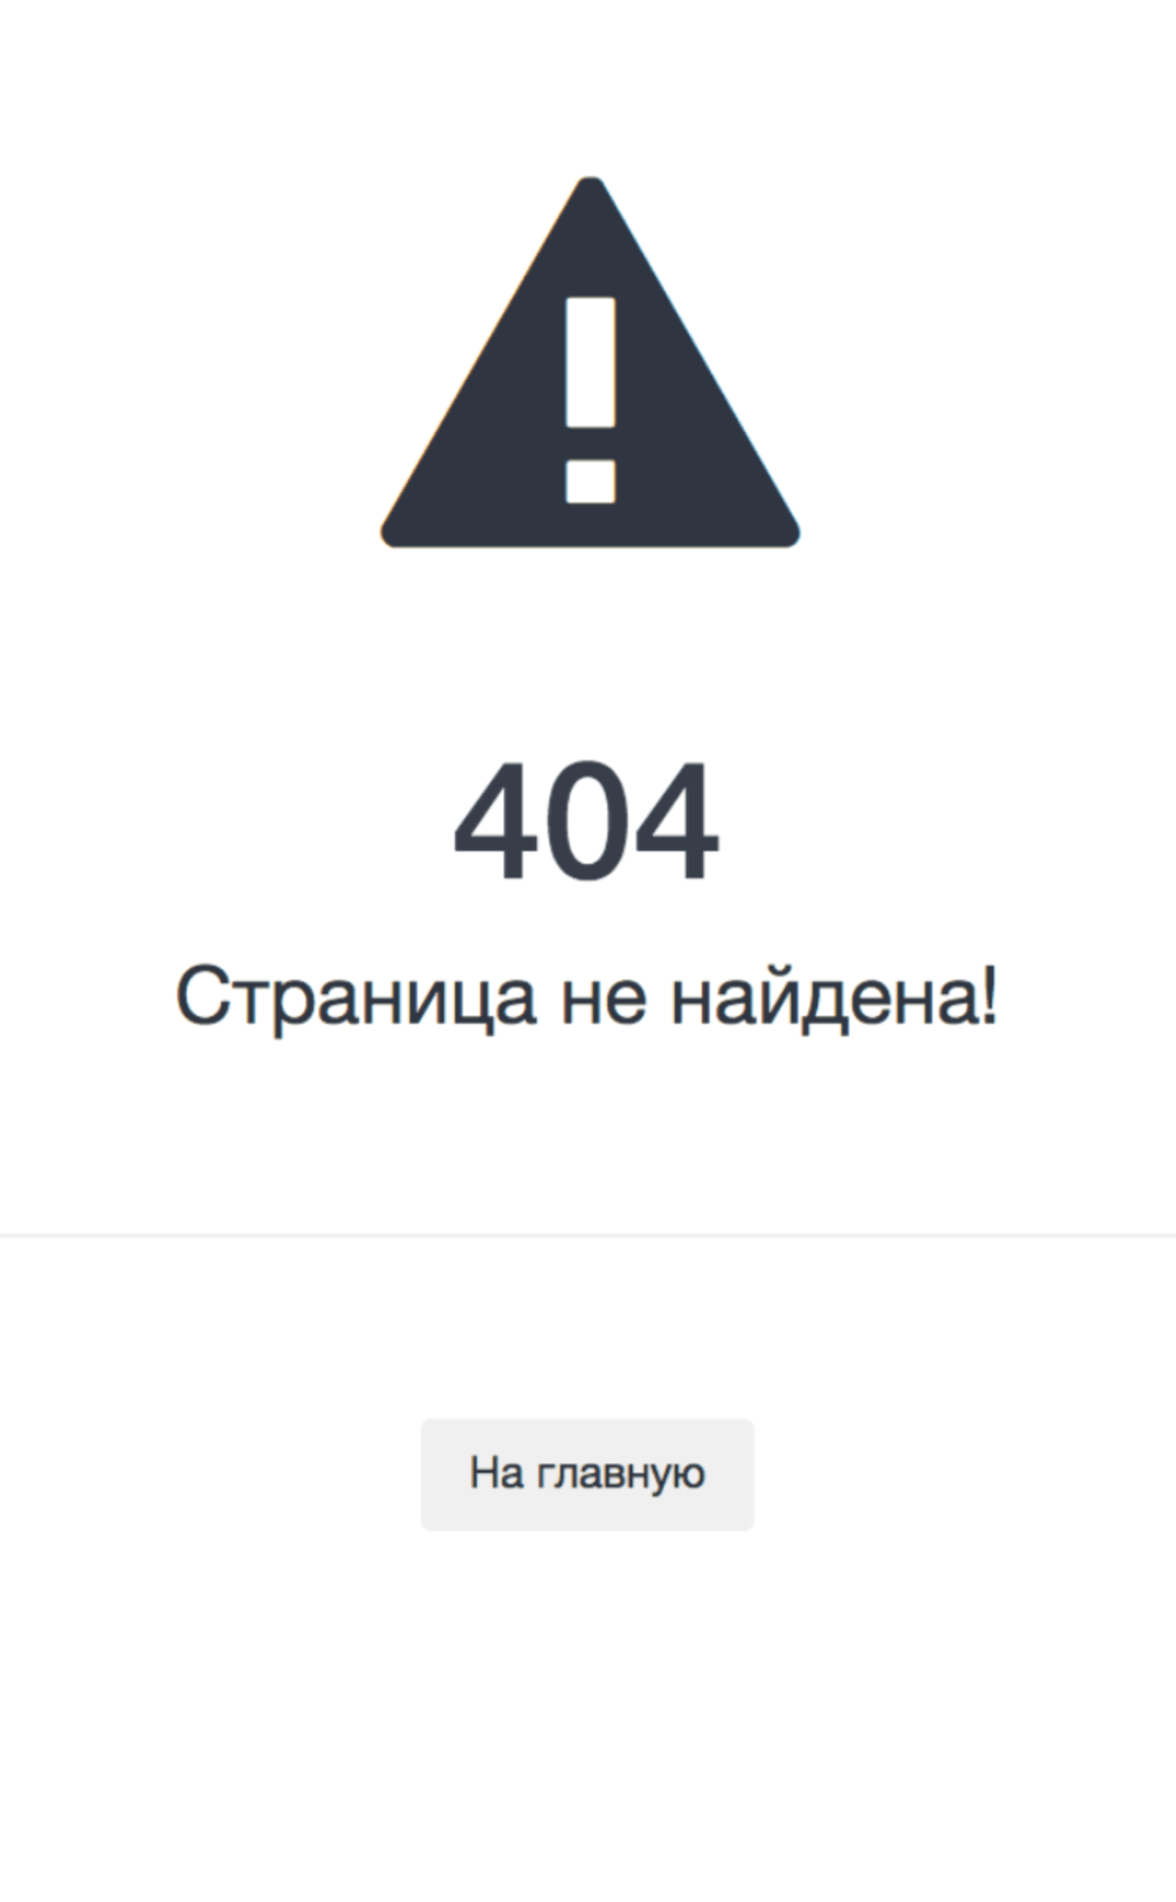
\includegraphics[width=0.35\textwidth]{figures/page_not_found}
         }
         \caption{Страницы в веб-сервисе “Spectral~Analyzer~PK-4”.: \pt(a) аутентификации, \pt(b) отсутствие страницы.}
         \label{fig:auth_and_page_not_found}
    \end{center}
\end{figure}

\begin{lstlisting}[style=py]
from django.contrib.auth.base_user import AbstractBaseUser
from django.contrib.auth.models import UserManager
from django.db import models

class User(AbstractBaseUser):
    email = models.EmailField(unique=True)
    first_name = models.CharField(max_length=64)
    last_name = models.CharField(max_length=64)
    institute = models.ForeignKey(Institute, models.DO_NOTHING)
    objects = UserManager()
    USERNAME_FIELD = "email"
\end{lstlisting}
У пользователя есть уникальная почта в системе, имя и фамилия, определена принадлежность к институту,
а также базовые параметры: хешированный пароль и время последней аутентификации.

На примере аутентификации разберем как происходят POST и GET запросы к удаленному веб-сервису, поскольку технически
данный подход ничем не отличается от получения информации по спектрам. Запрос GET используется для получения
содержимого указанного ресурса. С помощью метода GET можно также начать какой-либо процесс. Клиент может передавать
параметры выполнения запроса в URI целевого ресурса после символа «?»:
\begin{verbatim}
GET /login?param1=value1&param2=value2 HTTP/1.1
\end{verbatim}
Таким образом браузер выступает в роли клиента и выполняет GET запрос на удаленный сервер, который уже понимает специфику
HTTP протокола и предпринимает соответствующее действие. На примере аутентификации, при выполнении GET запроса должна
отобразиться страница, где, собственно, можно пройти аутентификацию (см.~рис.~\ref{sub:auth}). Для выполнения ответа
на данный запрос веб-сервис сверяет URL в соответствии со списком "urlpatterns":
\begin{lstlisting}[style=py]
from django.conf.urls import url
from web.views import LoginView

urlpatterns = [url(r"^login$", LoginView.as_view())]
\end{lstlisting}
Если не нашлось совпадения URL по регулярному выражению, то отоборажается ошибка 404 “Not Found” (см.~рис.~\ref{sub:page_not_found}),
а в случае совпадения выполняется действие, которое задается методом “get” класса LoginView:
\begin{lstlisting}[style=py]
from django.views.generic import View
from django.http import JsonResponse
from django.conf import settings
from django.shortcuts import render, redirect
from django.contrib.auth import authenticate, login, REDIRECT_FIELD_NAME

from web.models import User

class LoginView(View):

    def get(self, request):
        if request.user.is_authenticated:
            return redirect("/base")
        return render(request, "web/login.html")

    def post(self, request, redirect_field_name=REDIRECT_FIELD_NAME):
        def error(error_text):
            return JsonResponse({"error": error_text}, status=401)

        redirect_to = request.POST.get(redirect_field_name, settings.LOGIN_REDIRECT_URL)
        # Ensure the user-originating redirection url is safe.
        if not is_safe_url(url=redirect_to, host=request.get_host()):
            redirect_to = settings.LOGIN_REDIRECT_URL

        if "email" not in request.POST:
            return error("Email required")
        if "password" not in request.POST:
            return error("Password required")

        email = request.POST["email"].strip().lower()
        password = request.POST["password"]
        try:
            User.objects.get(email=email)
        except User.DoesNotExist:
            return error("Invalid email")

        user = authenticate(email=email, password=password)
        if user is None:
            return error("Invalid password")

        login(request, user)
        return JsonResponse({"redirect_url": redirect_to})
\end{lstlisting}
В методе “get” содержится логика, что если пользователь прошел аутентификацию, то не нужно требовать проходить ее еще раз,
а необходимо перенаправить на основную страницу. В случае если аутентификация не пройдена, то необходимо отобразить
html-страницу “web/login.html”.

В случае с POST запросами все немного сложнее. Они применяются для передачи пользовательских данных заданному ресурсу.
Логика с определением “команды для сервера” остается такой же, как и в GET запросе, но сам запрос отличается своей структурой:
данные необходимо передавать в тело запроса. Поскольку передача пользовательских данных требует безопасности, то
необходима защита. Например, в Джанго можно выставить требование на передачу CSRF-токена для любого POST-запроса.
Что это значит? CSRF-токен является последовательностью символов, которая передается вместе с ответом на GET запрос,
причем на каждый ответ сервер генерит новую последовательность, отличную от предыдущей. Если в POST запросе не был прислан
CSRF-токен или присланный токен не совпадает со сгенерированным сервером, то сервер отклоняется действие. Таким образом, можно
избежать межсайтовой подделки запроса и быть уверенными, что это реальный пользователь, а не злоумышленник.
На стороне клиента для совершения POST запросов в данном веб-сервисе используются
классические формы, после заполнения которых происходит POST-запрос, а также JQuery Ajax, если нет необходимости
перезагружать страницу для обновления данных:
\begin{figure}[t]
  \centering
  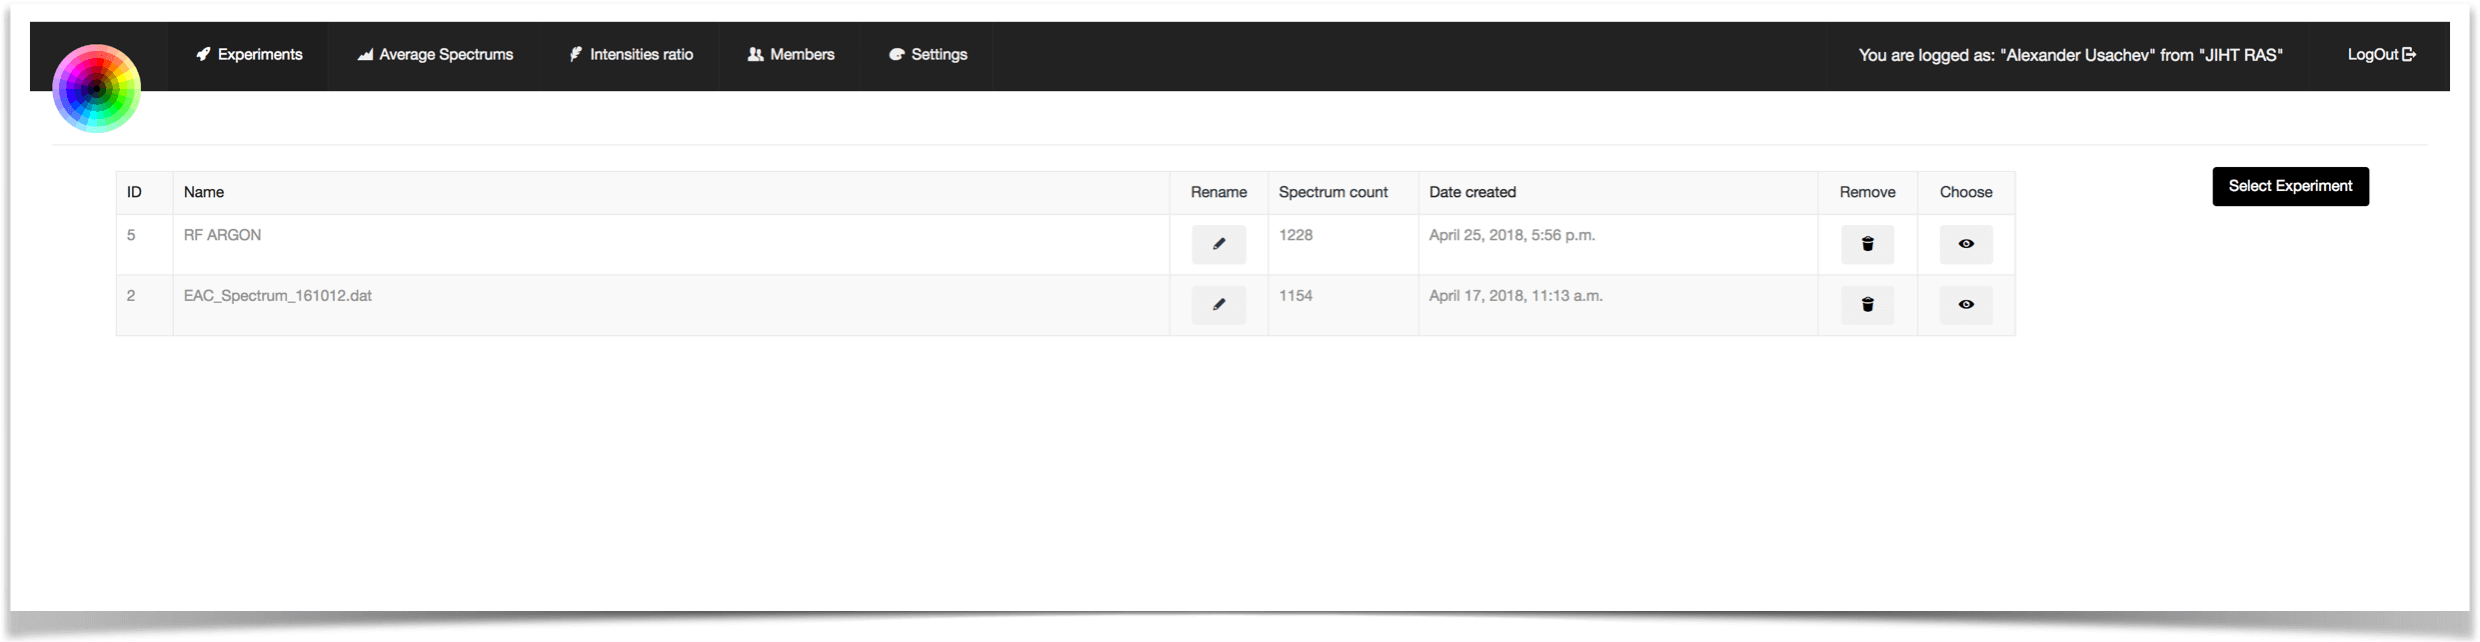
\includegraphics[width=16cm]{figures/all_experiments}
  \caption{Изображен результат рендеринга страницы “/all\_experiments” веб-сервиса “Spectral~Analyzer~PK-4”.}
  \label{fig:all_experiments}
\end{figure}
\begin{lstlisting}[style=htmlcssjs]
// Send data to the server
$.ajax({
    url: "/login",
    method: "POST",
    data: {
        email: $("input#email").val(),
        password: $("input#password").val(),
        next: $("input[name=next]").val(),
        csrfmiddlewaretoken: $("input[name=csrfmiddlewaretoken]").val(),
    },
    error: function(response) {
        <some_action>
    },
    success: function(response) {
        <some_action>
    }
});
\end{lstlisting}
Выполняя данный запрос, веб-сервис реагирует методом “post” класса “LoginView”, в котором содержится логика, что
если почта или пароль отстутсвуют, или, если нет пользователя с данной почтой, или пароль не совпадает, то аутентификация не пройдена
и надо это сообщить пользователю, а иначе перенаправить на основную страницу веб-сервиса.

Примерно на таком уровне проходит взаимодействие между пользователем и сервисом на программном уровне.
Необходимо придерживаться данных правил и задавать свои действия для методов “get” и “post” в соответствующем
наследнике класса “View”.

Итак, выполнив аутентификацию, пользователь попадает на основную страницу “Spectral~Analyzer~PK-4” с URL “/all\_experiments”
(см.~рис.~\ref{fig:all_experiments}), которая содержит:
\begin{itemize}
\item общее для всех меню, необходимое для навигации по сервису, в котором также содержится кнопка для выхода из системы,
а также имя, фамилия и институт авторизованного пользователя;
\item таблицу с уже загруженными экспериментами, в которой отображены ID, название, дата загрузки и количество спектров
в эксперименте. Также в таблице есть кнопки для переименования, удаления и просмотра эксперимента;
\item кнопку для загрузки и парсинга сырого файла со спектрами в формате “.dat”, данная процедура проводит запись в базу
данных;
\end{itemize}

Наибольший интерес из перечисленного представляет собой кнопка с загрузкой эксперимента, пример эксперимента можно найти в
\hyperref[app:app1]{приложении~А}. Под функционалом данной кнопки предполагается парсер спектральных блоков,
который умеет определять длины волн и интенсивности, а также метаинформацию из сырых данных. Ниже приведен
метод, который позволяет получить структуру файла в привычном для Python виде:
\begin{lstlisting}[style=py]
import re
from dateutil.parser import parse

def parse_raw_data(lines):
    spectrums = []
    metadata = []
    i = 0
    while i < len(lines) - 1:
        i += 1
        if re.match(r'##', lines[i]):
            if metadata:
                spectrums.append([parse_metadata(metadata),
                                  coordinates])
                metadata = []
        elif re.match(r'#', lines[i]):
            metadata.append(lines[i])
        elif re.match(r'0', lines[i]):
            coordinates = {x[:-1]: y for line in lines[i:i+2048]
                           for x, y in [line.split()]}
            i += 2047
    return spectrums

def parse_metadata(metadata):
    return {
        "started": parse(metadata[1].split()[2], yearfirst=True,
                         dayfirst=False),
        "hpc": re.findall(r"HPC=([0-9]{1,16})", metadata[2])[0],
        "hpc_freq": re.findall(r"HPCFreq=([0-9]{1,16})",
                               metadata[2])[0],
        "hpc_uptime": re.findall(r"HPC uptime = "
                                 "([0-9]{1,8}\.[0-9]{1,8})",
                                 metadata[2])[0],
        "spectrometer_commanded": parse(metadata[3].split()[1],
                                        yearfirst=True,
                                        dayfirst=False),
        "spectrometer_received": parse(metadata[4].split()[1],
                                       yearfirst=True,
                                       dayfirst=False),
        "start_marker": re.findall(r"([0-9]{1,16});",
                                   metadata[6])[0],
        "data_size_flag": re.findall(r"([0-9]{1,16});",
                                     metadata[7])[0],
        "nr_scans_accumulated": re.findall(r"([0-9]{1,16});",
                                           metadata[8])[0],
        "integration_time": re.findall(r"([0-9]{1,16});",
                                       metadata[9])[0],
        "fpga_esv_msw": re.findall(r"([0-9]{1,16});",
                                   metadata[10])[0],
        "fpga_esv_lsw": re.findall(r"([0-9]{1,16});",
                                   metadata[11])[0],
        "pixel_mode": re.findall(r"([0-9]{1,16});",
                                 metadata[12])[0],
        "end_marker": re.findall(r"([0-9]{1,16});",
                                 metadata[13])[0],
        "read_out_time": re.findall(
            r"time = ([0-9]{1,8}\.[0-9]{1,8})", metadata[14])[0],
        "ended": parse(metadata[15].split()[2], yearfirst=True,
                       dayfirst=False),
        "execution_time": re.findall(
            r"time = ([0-9]{1,8}\.[0-9]{1,8})", metadata[15])[0],
    }
\end{lstlisting}
\begin{figure}[t]
  \centering
  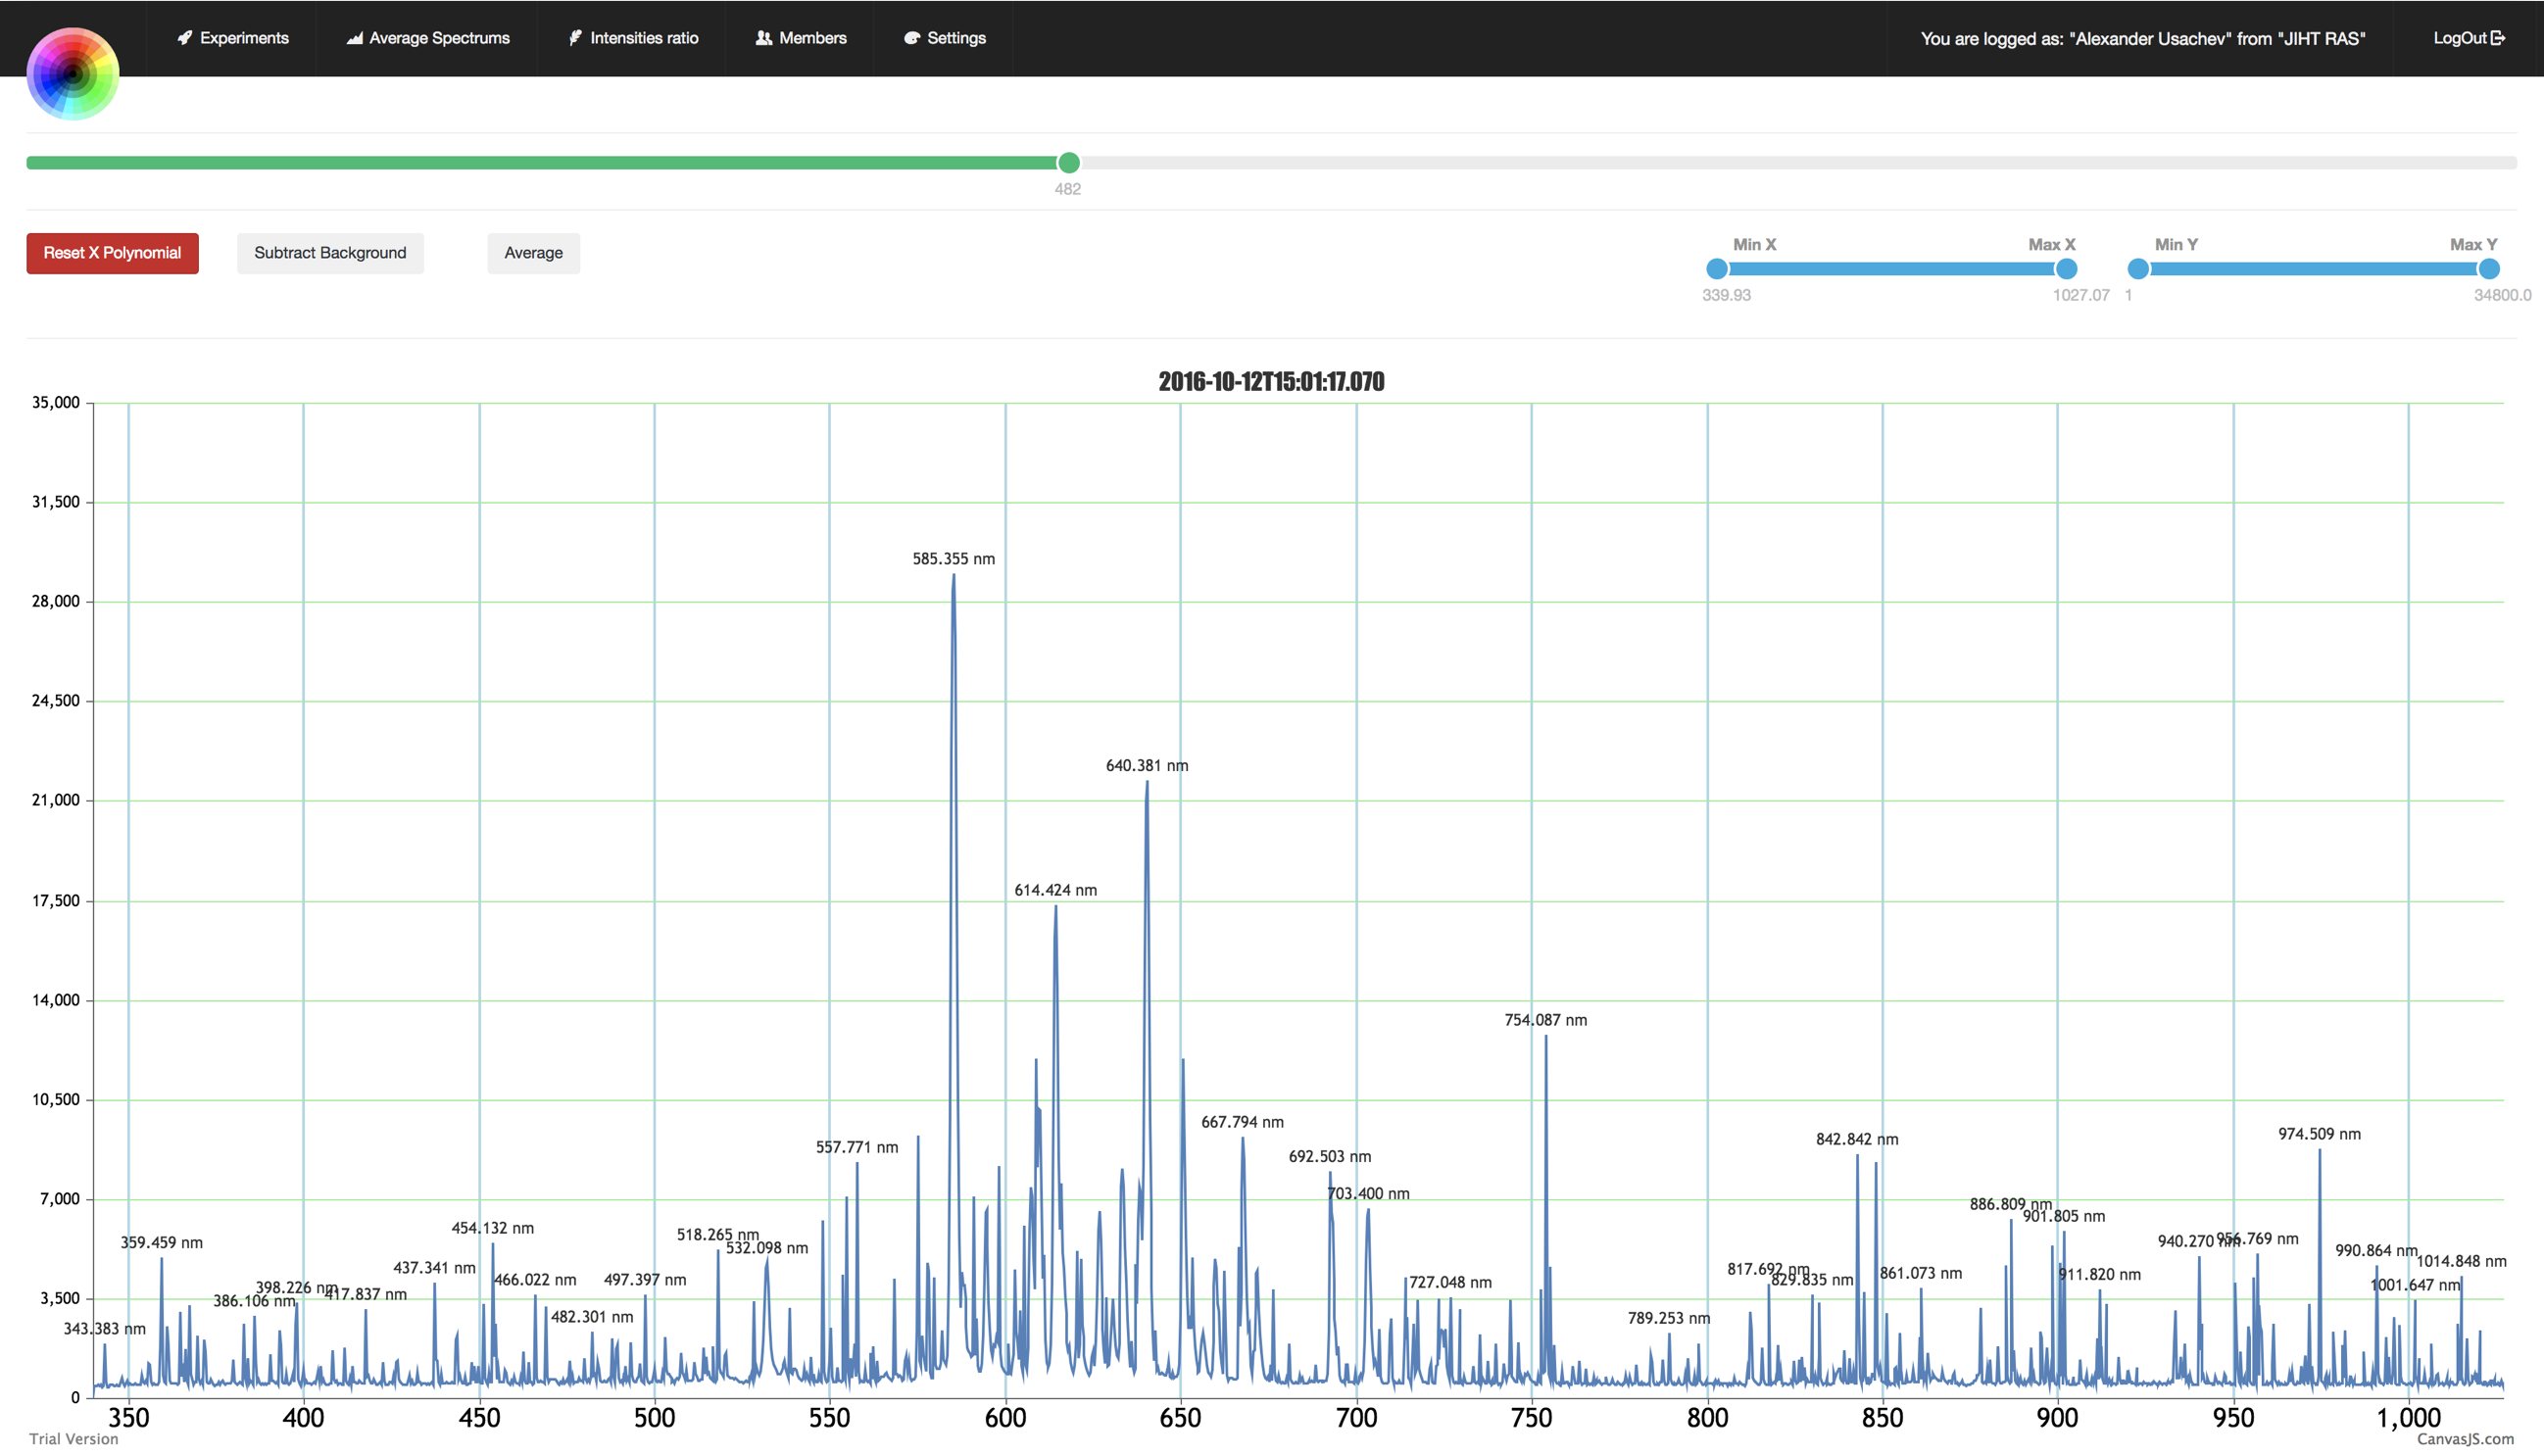
\includegraphics[width=16cm]{figures/experiment}
  \caption{Страница веб-сервиса “Spectral~Analyzer~PK-4”, на которой осуществляется просмотр спектров эксперимента.}
  \label{fig:experiment}
\end{figure}
Переменная “lines” является списком всех строк исходного файла. При загрузке файла с размером 32.1~Мб, который имеет
2385319 строк, метод “parse\_raw\_data” отрабатывает за время равное 1.81~с на среднем процессоре. Добавив логику с записью
информации в базу данных, получим рабочий скрипт по загрузке экспериментов.

После того, как эксперимент распознался и добавился на главную страницу, можно приступать к просмотру эксперимента.
Основную часть страницы занимает график со спектром: по оси абсцисс отложена длина волны в нм, по оси ординат интенсивность
спектральных линий в относительных единицах (см.~рис.~\ref{fig:experiment}). Для навигации по эксперименту используется слайдер,
размещенный вверху страницы. Передвигая бегунок, на программном уровне обновляется состояние переменной, отвечающей за номер спектра в эксперименте.
Проверка на обновление состояния графика происходит каждые 0.1~с, если была изменена одна из отслеживаемых переменных, то
с помощью JQuery Ajax отправляется POST запрос на сервер с целью получить координаты текущего спектра без обновления
страницы, а затем заново по ним отрисовывается график. По такому принципу и в дальнейшем будут работать любые обновления
графиков.

Чуть ниже справа находятся еще два слайдера, которые отвечают за масштабирование графика по осям X и Y: задаются
состояния переменных минимального и максимального значений для каждой из осей.

Слева расположены три кнопки, отвечающие за манипуляции с экспериментом:
\begin{itemize}
\item левая кнопка отвечает за настройку калибровки длинноволновой шкалы с помощью полинома пятой степени;
\item центральная кнопка отвечает за вычитание шумового фона по номерам выбранным спектров;
\item правая кнопка отвечает за сохранение усредненных выбранных спектров эксперимента для дальнейшей обработки.
\end{itemize}





























